%%%% Paramétrage du TD %%%%
\def\xxactivite{Colle \ifprof -- Corrigé \else \fi} % \normalsize \vspace{-.4cm}
\def\xxauteur{\textsl{Xavier Pessoles}}


\def\xxnumchapitre{Chapitre 1 \vspace{.2cm}}
\def\xxchapitre{\hspace{.12cm} Correction des systèmes}


\def\xxcompetences{%
\vspace{-.3cm}
\textsl{%
\textbf{Savoirs et compétences :}\\
\vspace{-.4cm}
\begin{itemize}[label=\ding{112},font=\color{ocre}] 
%\item \textit{Res1.C4 : } Correction
 \item \textit{Res1.C4.SF1 : } Proposer la démarche de réglage d’un correcteur proportionnel
%proportionnel intégral 
%et à avance de phase
\item \textit{Con.C2 : } 	Correction d’un système asservi	
\item \textit{Con.C2.SF1 : } Choisir un type de correcteur adapté
\end{itemize}
}}

\def\xxauteur{\textsl{Xavier Pessoles}}

\def\xxtitreexo{Véhicule à trois roues Clever \ifnormal $\star$ \else \fi \iftdifficile $\star\star\star$ \else \fi }
\def\xxsourceexo{\hspace{.2cm} \footnotesize{Banque PT -- SIA 2013}}

\def\xxfigures{
%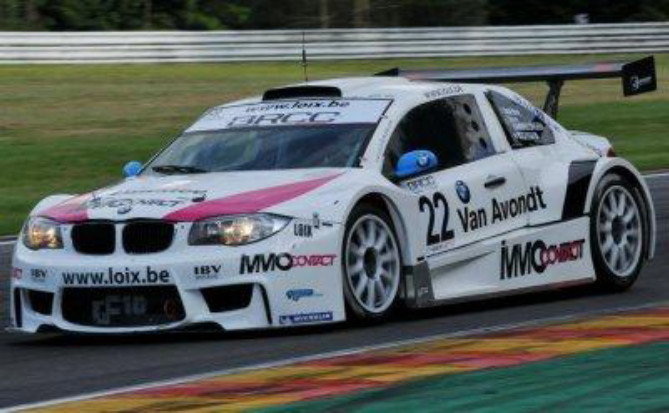
\includegraphics[width=.75\textwidth]{fig_00}
}%figues de la page de garde


\iflivret
\pagestyle{empty}


%%%%%%%% PAGE DE GARDE COURS
\ifcours
% ==== BANDEAU DES TITRES ==== 
\begin{tikzpicture}[remember picture,overlay]
\node at (current page.north west)
{\begin{tikzpicture}[remember picture,overlay]
\node[anchor=north west,inner sep=0pt] at (0,0) {\includegraphics[width=\paperwidth]{\thechapterimage}};
\draw[anchor=west] (-2cm,-8cm) node [line width=2pt,rounded corners=15pt,draw=ocre,fill=white,fill opacity=0.6,inner sep=40pt]{\strut\makebox[22cm]{}};
\draw[anchor=west] (1cm,-8cm) node {\huge\sffamily\bfseries\color{black} %
\begin{minipage}{1cm}
\rotatebox{90}{\LARGE\sffamily\textsc{\color{ocre}\textbf{\xxnumpartie}}}
\end{minipage} \hfill
\begin{minipage}[c]{14cm}
\begin{titrepartie}
\begin{flushright}
\renewcommand{\baselinestretch}{1.1} 
\Large\sffamily\textsc{\textbf{\xxpartie}}
\renewcommand{\baselinestretch}{1} 
\end{flushright}
\end{titrepartie}
\end{minipage} \hfill
\begin{minipage}[c]{3.5cm}
{\large\sffamily\textsc{\textbf{\color{ocre} \discipline}}}
\end{minipage} 
 };
\end{tikzpicture}};
\end{tikzpicture}
% ==== FIN BANDEAU DES TITRES ==== 


% ==== ONGLET 
\begin{tikzpicture}[overlay]
\node[shape=rectangle, 
      rounded corners = .25 cm,
	  draw= ocre,
	  line width=2pt, 
	  fill = ocre!10,
	  minimum width  = 2.5cm,
	  minimum height = 3cm,] at (18.3cm,0) {};
\node at (17.7cm,0) {\rotatebox{90}{\textbf{\Large\color{ocre}{\classe}}}};
%{};
\end{tikzpicture}
% ==== FIN ONGLET 


\vspace{3.5cm}

\begin{tikzpicture}[remember picture,overlay]
\draw[anchor=west] (-2cm,-6cm) node {\huge\sffamily\bfseries\color{black} %
\begin{minipage}{2cm}
\begin{center}
\LARGE\sffamily\textsc{\color{ocre}\textbf{\xxactivite}}
\end{center}
\end{minipage} \hfill
\begin{minipage}[c]{15cm}
\begin{titrechapitre}
\renewcommand{\baselinestretch}{1.1} 
\Large\sffamily\textsc{\textbf{\xxnumchapitre}}

\Large\sffamily\textsc{\textbf{\xxchapitre}}
\vspace{.5cm}

\renewcommand{\baselinestretch}{1} 
\normalsize\normalfont
\xxcompetences
\end{titrechapitre}
\end{minipage}  };
\end{tikzpicture}
\vfill

\begin{flushright}
\begin{minipage}[c]{.3\linewidth}
\begin{center}
\xxfigures
\end{center}
\end{minipage}\hfill
\begin{minipage}[c]{.6\linewidth}
\startcontents
%\printcontents{}{1}{}
\printcontents{}{1}{}
\end{minipage}
\end{flushright}

\begin{tikzpicture}[remember picture,overlay]
\draw[anchor=west] (4.5cm,-.7cm) node {
\begin{minipage}[c]{.2\linewidth}
\begin{flushright}

\includegraphics[width=2cm]{logoCC}
\end{flushright}
\end{minipage}
\begin{minipage}[c]{.2\linewidth}
\textsl{\xxauteur} \\
\textsl{\classe}
\end{minipage}
 };
\end{tikzpicture}

\newpage
\pagestyle{fancy}

%\newpage
%\pagestyle{fancy}

\else
\fi
%% FIN PAGE DE GARDE DES COURS

%%%%%%%% PAGE DE GARDE TD
\iftd

% BANDEAU EXO
\iflivret % SI LIVRET ET TD
\begin{tikzpicture}[remember picture,overlay]
\draw[anchor=west] (-2cm,-3.3cm) node {\huge\sffamily\bfseries\color{black} %
\begin{minipage}{5cm}
\begin{center}
\LARGE\sffamily\color{ocre}\textbf{\textsc{\xxactivite}}

\begin{center}
\xxfigures
\end{center}

\end{center}
\end{minipage} \hfill
\begin{minipage}[c]{12cm}
\begin{titrechapitre}
\renewcommand{\baselinestretch}{1.1} 
\large\sffamily\textbf{\textsc{\xxtitreexo}}

\small\sffamily{\textbf{\textit{\color{black!70}\xxsourceexo}}}
\vspace{.5cm}

\renewcommand{\baselinestretch}{1} 
\normalsize\normalfont
\xxcompetences
\end{titrechapitre}
\end{minipage}};
\end{tikzpicture}
\else % ELSE NOT LIVRET
\begin{tikzpicture}[remember picture,overlay]
\draw[anchor=west] (-2cm,-3.5cm) node {\huge\sffamily\bfseries\color{black} %
\begin{minipage}{5cm}
\begin{center}
\LARGE\sffamily\color{ocre}\textbf{\textsc{\xxactivite}}

\begin{center}
\xxfigures
\end{center}

\end{center}
\end{minipage} \hfill
\begin{minipage}[c]{12cm}
\begin{titrechapitre}
\renewcommand{\baselinestretch}{1.1} 
\large\sffamily\textbf{\textsc{\xxtitreexo}}

\small\sffamily{\textbf{\textit{\color{black!70}\xxsourceexo}}}
\vspace{.5cm}

\renewcommand{\baselinestretch}{1} 
\normalsize\normalfont
\xxcompetences
\end{titrechapitre}
\end{minipage}};
\end{tikzpicture}

\fi

\else   % FIN IF TD
\fi


%%%%%%%% PAGE DE GARDE FICHE
\iffiche
\begin{tikzpicture}[remember picture,overlay]
\node at (current page.north west)
{\begin{tikzpicture}[remember picture,overlay]
\draw[anchor=west] (-2cm,\xxYCartouche) node [line width=2pt,rounded corners=15pt,draw=ocre,fill=white,fill opacity=0.6,inner sep=40pt]{\strut\makebox[22cm]{}};
\draw[anchor=west] (1cm,\xxYCartouche) node {\huge\sffamily\bfseries\color{black} %
\begin{minipage}{1cm}
\rotatebox{90}{\LARGE\sffamily\textsc{\color{ocre}\textbf{\xxnumpartie}}}
\end{minipage} \hfill
\begin{minipage}[c]{14cm}
\begin{titrepartie}
\begin{flushright}
\renewcommand{\baselinestretch}{1.1} 
\large\sffamily\textsc{\textbf{\xxpartie} \\} 

\vspace{.2cm}

\normalsize\sffamily\textsc{\textbf{\xxnumchapitre -- \xxchapitre}}
\renewcommand{\baselinestretch}{1} 
\end{flushright}
\end{titrepartie}
\end{minipage} \hfill
\begin{minipage}[c]{3.5cm}
{\large\sffamily\textsc{\textbf{\color{ocre} \discipline}}}
\end{minipage} 
 };
\end{tikzpicture}};
\end{tikzpicture}

\iflivret % SI LIVRET
\begin{tikzpicture}[overlay]
\node[shape=rectangle, 
      rounded corners = .25 cm,
	  draw= ocre,
	  line width=2pt, 
	  fill = ocre!10,
	  minimum width  = 2.5cm,
	  minimum height = 2.5cm,] at (18.5cm,\xxYongletGarde) {};
\node at (17.9cm,\xxYongletGarde) {\rotatebox{90}{\textsf{\textbf{\large\color{ocre}{\classe}}}}};
%{};
\end{tikzpicture}
\else  % SI PAS LIVRET
\iftd %% SI TD et PAS LIVRET
\begin{tikzpicture}[overlay]
\node[shape=rectangle, 
      rounded corners = .25 cm,
	  draw= ocre,
	  line width=2pt, 
	  fill = ocre!10,
	  minimum width  = 2.5cm,
	  minimum height = 2.5cm,] at (18.6cm,\xxYOnget) {}; %% 0.9 par défaut
\node at (18cm,\xxYOnget) {\rotatebox{90}{\textsf{\textbf{\large\color{ocre}{\classe}}}}};
%{};
\end{tikzpicture}

\else % FIN DU SI TD PAS LIVRET 
\begin{tikzpicture}[overlay]
\node[shape=rectangle, 
      rounded corners = .25 cm,
	  draw= ocre,
	  line width=2pt, 
	  fill = ocre!10,
	  minimum width  = 2.5cm,
%	  minimum height = 2.5cm,] at (18.5cm,1.1cm) {}; % \xxYOnget 0.5
	  minimum height = 2.5cm,] at (18.6cm,.5cm) {};
\node at (18cm,.5cm) {\rotatebox{90}{\textsf{\textbf{\large\color{ocre}{\classe}}}}};
%{};
\end{tikzpicture}
\fi
\fi
\else
\fi



\else
\pagestyle{empty}


%%%%%%%% PAGE DE GARDE COURS
\ifcours
% ==== BANDEAU DES TITRES ==== 
\begin{tikzpicture}[remember picture,overlay]
\node at (current page.north west)
{\begin{tikzpicture}[remember picture,overlay]
\node[anchor=north west,inner sep=0pt] at (0,0) {\includegraphics[width=\paperwidth]{\thechapterimage}};
\draw[anchor=west] (-2cm,-8cm) node [line width=2pt,rounded corners=15pt,draw=ocre,fill=white,fill opacity=0.6,inner sep=40pt]{\strut\makebox[22cm]{}};
\draw[anchor=west] (1cm,-8cm) node {\huge\sffamily\bfseries\color{black} %
\begin{minipage}{1cm}
\rotatebox{90}{\LARGE\sffamily\textsc{\color{ocre}\textbf{\xxnumpartie}}}
\end{minipage} \hfill
\begin{minipage}[c]{14cm}
\begin{titrepartie}
\begin{flushright}
\renewcommand{\baselinestretch}{1.1} 
\Large\sffamily\textsc{\textbf{\xxpartie}}
\renewcommand{\baselinestretch}{1} 
\end{flushright}
\end{titrepartie}
\end{minipage} \hfill
\begin{minipage}[c]{3.5cm}
{\large\sffamily\textsc{\textbf{\color{ocre} \discipline}}}
\end{minipage} 
 };
\end{tikzpicture}};
\end{tikzpicture}
% ==== FIN BANDEAU DES TITRES ==== 


% ==== ONGLET 
\begin{tikzpicture}[overlay]
\node[shape=rectangle, 
      rounded corners = .25 cm,
	  draw= ocre,
	  line width=2pt, 
	  fill = ocre!10,
	  minimum width  = 2.5cm,
	  minimum height = 3cm,] at (18.3cm,0) {};
\node at (17.7cm,0) {\rotatebox{90}{\textbf{\Large\color{ocre}{\classe}}}};
%{};
\end{tikzpicture}
% ==== FIN ONGLET 


\vspace{3.5cm}

\begin{tikzpicture}[remember picture,overlay]
\draw[anchor=west] (-2cm,-6cm) node {\huge\sffamily\bfseries\color{black} %
\begin{minipage}{2cm}
\begin{center}
\LARGE\sffamily\textsc{\color{ocre}\textbf{\xxactivite}}
\end{center}
\end{minipage} \hfill
\begin{minipage}[c]{15cm}
\begin{titrechapitre}
\renewcommand{\baselinestretch}{1.1} 
\Large\sffamily\textsc{\textbf{\xxnumchapitre}}

\Large\sffamily\textsc{\textbf{\xxchapitre}}
\vspace{.5cm}

\renewcommand{\baselinestretch}{1} 
\normalsize\normalfont
\xxcompetences
\end{titrechapitre}
\end{minipage}  };
\end{tikzpicture}
\vfill

\begin{flushright}
\begin{minipage}[c]{.3\linewidth}
\begin{center}
\xxfigures
\end{center}
\end{minipage}\hfill
\begin{minipage}[c]{.6\linewidth}
\startcontents
%\printcontents{}{1}{}
\printcontents{}{1}{}
\end{minipage}
\end{flushright}

\begin{tikzpicture}[remember picture,overlay]
\draw[anchor=west] (4.5cm,-.7cm) node {
\begin{minipage}[c]{.2\linewidth}
\begin{flushright}

\includegraphics[width=2cm]{logoCC}
\end{flushright}
\end{minipage}
\begin{minipage}[c]{.2\linewidth}
\textsl{\xxauteur} \\
\textsl{\classe}
\end{minipage}
 };
\end{tikzpicture}

\newpage
\pagestyle{fancy}

%\newpage
%\pagestyle{fancy}

\else
\fi
%% FIN PAGE DE GARDE DES COURS

%%%%%%%% PAGE DE GARDE TD
\iftd

% BANDEAU EXO
\iflivret % SI LIVRET ET TD
\begin{tikzpicture}[remember picture,overlay]
\draw[anchor=west] (-2cm,-3.3cm) node {\huge\sffamily\bfseries\color{black} %
\begin{minipage}{5cm}
\begin{center}
\LARGE\sffamily\color{ocre}\textbf{\textsc{\xxactivite}}

\begin{center}
\xxfigures
\end{center}

\end{center}
\end{minipage} \hfill
\begin{minipage}[c]{12cm}
\begin{titrechapitre}
\renewcommand{\baselinestretch}{1.1} 
\large\sffamily\textbf{\textsc{\xxtitreexo}}

\small\sffamily{\textbf{\textit{\color{black!70}\xxsourceexo}}}
\vspace{.5cm}

\renewcommand{\baselinestretch}{1} 
\normalsize\normalfont
\xxcompetences
\end{titrechapitre}
\end{minipage}};
\end{tikzpicture}
\else % ELSE NOT LIVRET
\begin{tikzpicture}[remember picture,overlay]
\draw[anchor=west] (-2cm,-3.5cm) node {\huge\sffamily\bfseries\color{black} %
\begin{minipage}{5cm}
\begin{center}
\LARGE\sffamily\color{ocre}\textbf{\textsc{\xxactivite}}

\begin{center}
\xxfigures
\end{center}

\end{center}
\end{minipage} \hfill
\begin{minipage}[c]{12cm}
\begin{titrechapitre}
\renewcommand{\baselinestretch}{1.1} 
\large\sffamily\textbf{\textsc{\xxtitreexo}}

\small\sffamily{\textbf{\textit{\color{black!70}\xxsourceexo}}}
\vspace{.5cm}

\renewcommand{\baselinestretch}{1} 
\normalsize\normalfont
\xxcompetences
\end{titrechapitre}
\end{minipage}};
\end{tikzpicture}

\fi

\else   % FIN IF TD
\fi


%%%%%%%% PAGE DE GARDE FICHE
\iffiche
\begin{tikzpicture}[remember picture,overlay]
\node at (current page.north west)
{\begin{tikzpicture}[remember picture,overlay]
\draw[anchor=west] (-2cm,\xxYCartouche) node [line width=2pt,rounded corners=15pt,draw=ocre,fill=white,fill opacity=0.6,inner sep=40pt]{\strut\makebox[22cm]{}};
\draw[anchor=west] (1cm,\xxYCartouche) node {\huge\sffamily\bfseries\color{black} %
\begin{minipage}{1cm}
\rotatebox{90}{\LARGE\sffamily\textsc{\color{ocre}\textbf{\xxnumpartie}}}
\end{minipage} \hfill
\begin{minipage}[c]{14cm}
\begin{titrepartie}
\begin{flushright}
\renewcommand{\baselinestretch}{1.1} 
\large\sffamily\textsc{\textbf{\xxpartie} \\} 

\vspace{.2cm}

\normalsize\sffamily\textsc{\textbf{\xxnumchapitre -- \xxchapitre}}
\renewcommand{\baselinestretch}{1} 
\end{flushright}
\end{titrepartie}
\end{minipage} \hfill
\begin{minipage}[c]{3.5cm}
{\large\sffamily\textsc{\textbf{\color{ocre} \discipline}}}
\end{minipage} 
 };
\end{tikzpicture}};
\end{tikzpicture}

\iflivret % SI LIVRET
\begin{tikzpicture}[overlay]
\node[shape=rectangle, 
      rounded corners = .25 cm,
	  draw= ocre,
	  line width=2pt, 
	  fill = ocre!10,
	  minimum width  = 2.5cm,
	  minimum height = 2.5cm,] at (18.5cm,\xxYongletGarde) {};
\node at (17.9cm,\xxYongletGarde) {\rotatebox{90}{\textsf{\textbf{\large\color{ocre}{\classe}}}}};
%{};
\end{tikzpicture}
\else  % SI PAS LIVRET
\iftd %% SI TD et PAS LIVRET
\begin{tikzpicture}[overlay]
\node[shape=rectangle, 
      rounded corners = .25 cm,
	  draw= ocre,
	  line width=2pt, 
	  fill = ocre!10,
	  minimum width  = 2.5cm,
	  minimum height = 2.5cm,] at (18.6cm,\xxYOnget) {}; %% 0.9 par défaut
\node at (18cm,\xxYOnget) {\rotatebox{90}{\textsf{\textbf{\large\color{ocre}{\classe}}}}};
%{};
\end{tikzpicture}

\else % FIN DU SI TD PAS LIVRET 
\begin{tikzpicture}[overlay]
\node[shape=rectangle, 
      rounded corners = .25 cm,
	  draw= ocre,
	  line width=2pt, 
	  fill = ocre!10,
	  minimum width  = 2.5cm,
%	  minimum height = 2.5cm,] at (18.5cm,1.1cm) {}; % \xxYOnget 0.5
	  minimum height = 2.5cm,] at (18.6cm,.5cm) {};
\node at (18cm,.5cm) {\rotatebox{90}{\textsf{\textbf{\large\color{ocre}{\classe}}}}};
%{};
\end{tikzpicture}
\fi
\fi
\else
\fi



\fi
\setlength{\columnseprule}{.1pt}

\pagestyle{fancy}
\thispagestyle{plain}

\vspace{4.5cm}

\def\columnseprulecolor{\color{ocre}}
\setlength{\columnseprule}{0.4pt} 

\setcounter{exo}{0}

\ifprof
\begin{multicols}{2}
\else
\begin{multicols}{2}
\fi
%%%%%%%%%%%%%%%%%%%%%%%%%%%%%%%%%%%%%%%%%%%%%%%%%%
\subsection*{Présentation}

Le Clever est un démonstrateur technologique développé par un tissu d'industriels européens. Clever est la contraction de Compact Low Emission VEhiclefor uRban tRansportation (véhicule compacte à faibles émissions pour le transport urbain) car, avec une consommation de seulement \SI{2,5}{L}/\SI{100}{km}, il s'annonce très écologique. 

L'habitacle peut s'incliner grâce à un système constitué 
\begin{itemize}
\item d'un calculateur qui détermine le mouvement et la position à donner à l'habitacle en fonction des conditions d'utilisation ;
\item d'un système hydro-mécanique de transmission de puissance et d'adaptation de mouvement ;
\item d'un système de contrôle de l'inclinaison de l'habitacle.
\end{itemize}

\begin{center}
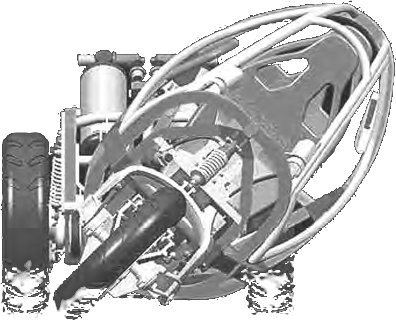
\includegraphics[width=.47\linewidth]{images/fig_02}
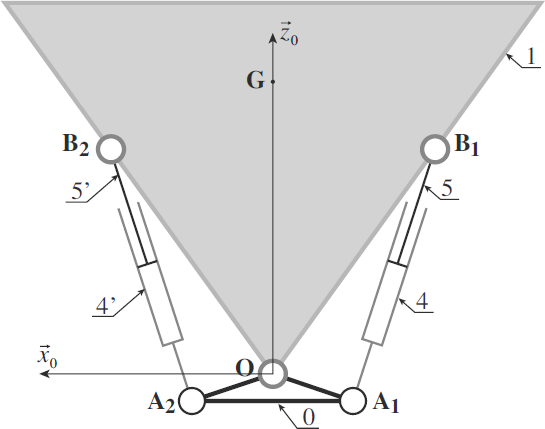
\includegraphics[width=.47\linewidth]{images/fig_03}
%\textit{}
\end{center}

%La chaîne de transmission de puissance et d'adaptation de mouvement est composée :
%\begin{itemize}
%\item d'une pompe à engrenages actionnée par le moteur à gaz via un système de poulies/courroie ;
%\item d'un circuit hydraulique ;
%\item de 2 vérins hydrauliques simple effet ;
%\item d'un système mécanique d'adaptation de mouvement afin de transformer le mouvement de translation des tiges des vérins en rotation de l'habitacle.
%\end{itemize}
\begin{obj}
L'objectif est que le mouvement de l'habitacle soit contrôlé :
\begin{itemize}
\item écart statique : 0\degres;
\item écart de traînage pour une entrée en rampe unitaire : 0\degres;
\item temps de réponse à 5\% : inférieur à \SI{0,1}{s}.

\end{itemize}
\end{obj}

\subsection*{Modélisation du servo-distributeur et du vérin}

L'orientation de l'habitacle est contrôlée par un asservissement de la position angulaire. L'architecture de cet asservissement est représentée par le schéma-blocs de le figure suivante.

On modélise le comportement du servo-distributeur par un gain pur noté $K_s$ et le capteur par $H_c(p)=C$ avec $C=\SI{1}{V.rad^{-1}}$.  L'adaptateur mécanique a un comportement linéaire sur l'intervalle d'utilisation. On a donc $H_{\text{am}}(p)=R$ ($R=\SI{7}{rad.m^{-1}}$). Enfin, on considère que $H_r(p)=1$. 

\begin{center}
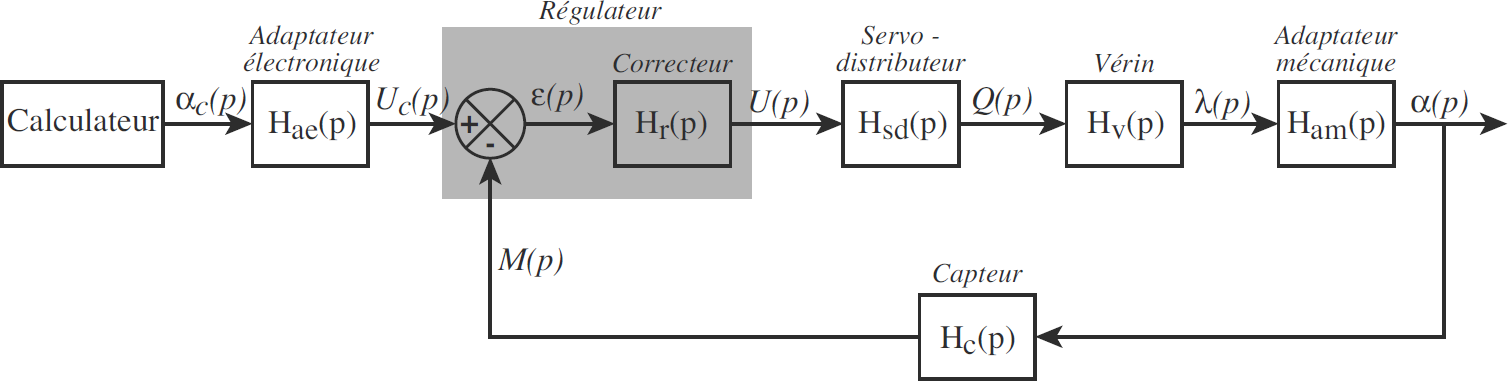
\includegraphics[width=\linewidth]{images/fig_05}
\captionof{figure}{Architecture générale du contrôle de l'orientation de l'habitacle \label{figii.3}}
\end{center}

À ce stade de l'étude, le modèle de comportement du fluide correspond à un comportement incompressible. L'équation caractérisant le comportement du vérin est alors : $q(t)=S\dot{\lambda}(t)$ où :
\begin{itemize}
\item $S$ représente la section utile du vérin en sortie de tige (diamètre \SI{32}{mm});
\item $q$ est le débit en entrée de vérin ;
\item $v(t)=\dot{\lambda}(t)=\dfrac{\dd \lambda(t) }{\dd t}$ est la vitesse de translation de la tige du vérin par rapport au corps.
\end{itemize}
% 

\subparagraph{}\textit{Donner l'expression de la fonction de transfert du vérin $H_{V1}(p)$ (telle que $\lambda(p) = H_{V1}(p) Q(p)$) et compléter le schéma-bloc associé à la modélisation actuelle du système.}
\ifprof
\begin{corrige} ~\\

\begin{center}
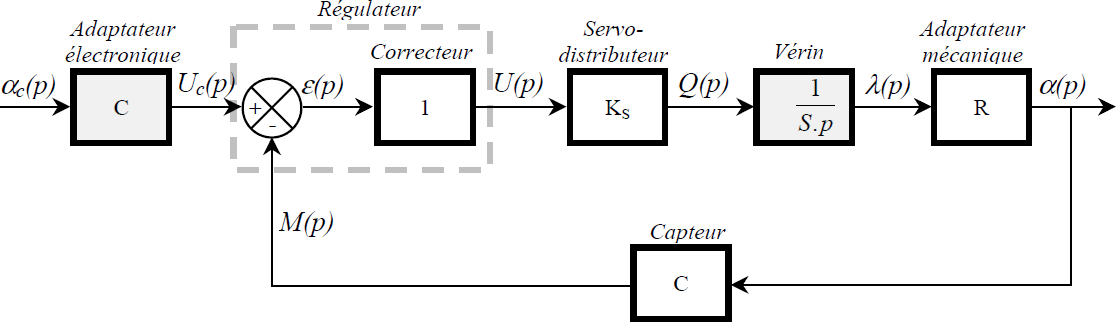
\includegraphics[width=.95\linewidth]{images/cor_01}
%\textit{}
\end{center}
\end{corrige}
\else
\fi

\subparagraph{}\textit{Déterminer la fonction de transfert en boucle fermée $\text{FTBF}_1$ (telle que $\alpha(p) = \text{FTBF}_1(p) \alpha_c(p)$) du système bouclé. Mettre  $\text{FTBF}_1(p)$ sous la forme 
$\dfrac{K_1}{1+\tau_1 p}$ en précisant les expressions de $K_1$ et de $\tau_1$.} 
 \ifprof
\begin{corrige} ~\\

\begin{center}
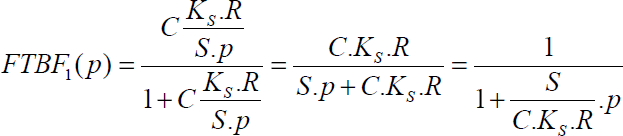
\includegraphics[width=.95\linewidth]{images/cor_02}
%\textit{}
\end{center}
\end{corrige}
\else
\fi


\subparagraph{}\textit{À partir du critère de temps de réponse à 5\% $(t_{r5\%})$ du système, déterminer l'expression puis la valeur numérique minimale du gain du servo-distributeur.} 

\ifprof
\begin{corrige}~\\
\begin{center}
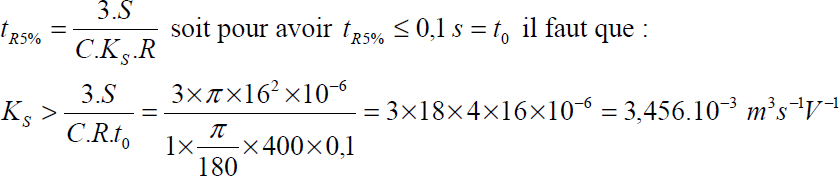
\includegraphics[width=.95\linewidth]{images/cor_03}
%\textit{}
\end{center}    
\end{corrige}
\else
\fi

\subsection*{Analyse des caractéristiques prévues par le modèle}


On cherche ici à déterminer les caractéristiques de la régulation de la position angulaire de l'habitacle prévu par le modèle construit précédemment.

\subparagraph{}\textit{Déterminer l'écart de traînage $\varepsilon_{\text{tr}}$ prévu par le modèle actuel. Le cahier des charges est-il satisfait ?} 
\ifprof
\begin{corrige}~\\
\end{corrige}
\else
\fi


On place un intégrateur dans le régulateur. On a alors : $H_r(p)=\dfrac{1}{p}$.
 

\subparagraph{}\textit{Le critère d'écart de traînage est-il satisfait ?} 
\ifprof
\begin{corrige}~\\
\end{corrige}
\else
\fi

\subparagraph{}\textit{Donner la valeur de la marge de phase. Conclure.} 
\ifprof
\begin{corrige}~\\
\end{corrige}
\else
\fi


\subsection*{Modélisation du comportement du vérin avec fluide compressible et du comportement dynamique du mécanisme}

La compressibilité du fluide étant prise en compte dans le modèle, l'évolution du débit est une fonction du déplacement mais aussi de la pression sous la forme de la relation (1). L'effort exercé par le vérin en sortie de tige est décrit par la relation (2).
$$
q(t)=S\dot{\lambda}(t)+\dfrac{V_0}{B}\dot{p}_r(t) \quad (1) \quad\quad
F_V(t)=Sp_r(t) \quad (2)
$$
où:
\begin{itemize}
\item $p_r(t)$ : pression utile dans le vérin ;
\item $V_0$ : volume caractéristique moyen de fluide contenu dans le vérin et les durites, $V_0 = \SI{2,5e5}{m^3}$;
\item $B$ : coefficient de compressibilité du fluide, $B = \SI{109}{Pa}$;
\item $F_v(t)$ : effort développé par le vérin en sortie de tige ;
\item $S$ : section utile du vérin en sortie de tige.
\end{itemize}

Par ailleurs, $F_v(t)+k_g \lambda(t)=m_{\text{eq}}\ddot{\lambda}(t)$ avec $m_{\text{eq}}$ la masse équivalente du système, $k_g$ une constante, $\lambda(t)$ le déploiement des vérins.



\subparagraph{}\textit{Appliquer la transformation de Laplace aux équations précédentes et compléter le schéma-blocs.}
\ifprof
\begin{corrige}
\begin{center}
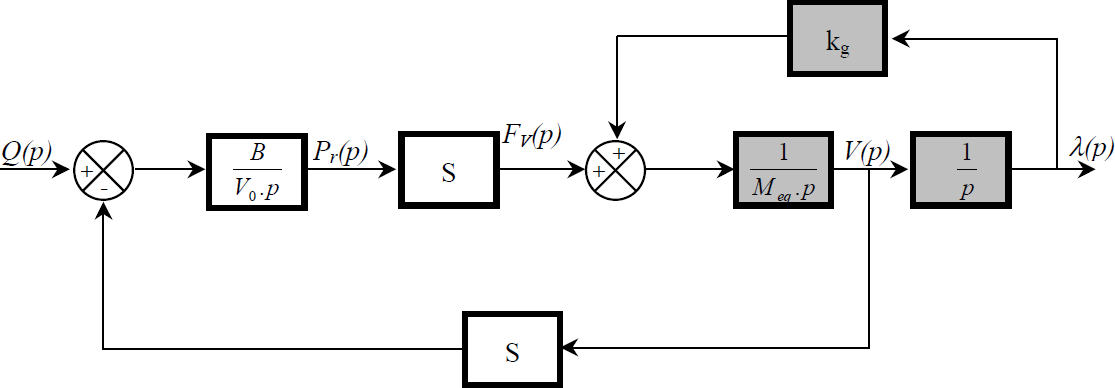
\includegraphics[width=.95\linewidth]{images/cor_04}
%\textit{}
\end{center}    
\end{corrige}
\else
\fi
%\begin{center}
%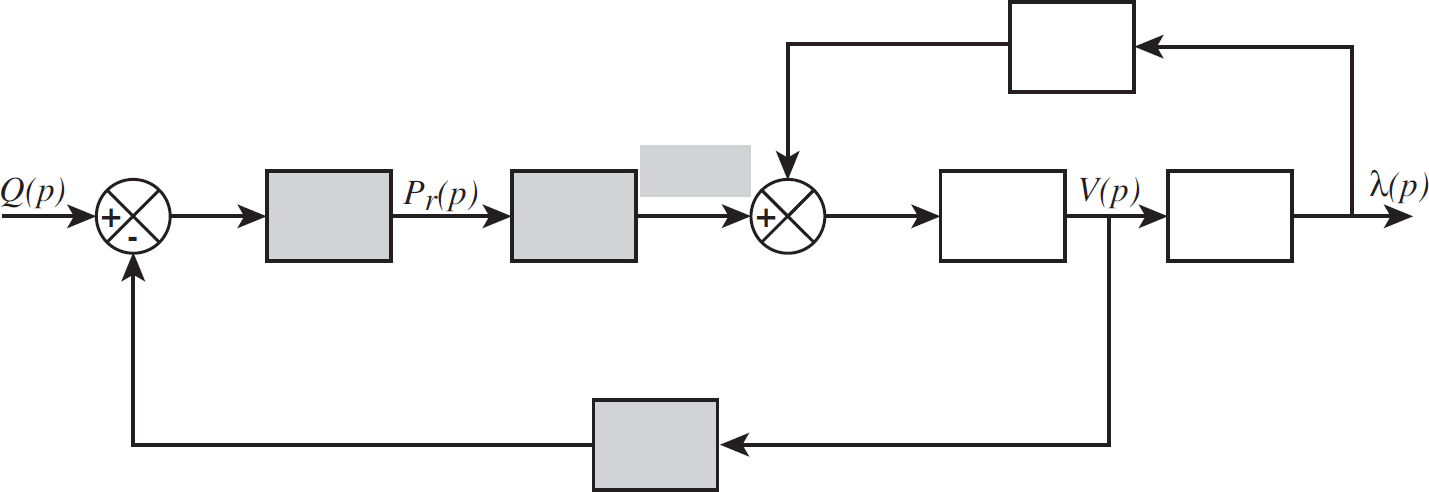
\includegraphics[width=\linewidth]{images/fig_06}
%%\textit{}
%\end{center}


\subsection*{Analyse du comportement global}


\subparagraph{}\textit{Donner l'expression de la fonction de transfert en boucle fermée du vérin $H_{\text{V2}}$ (telle que $\lambda(p) =  H_{\text{V2}} Q(p)$) et préciser les expressions des coefficients $K_V$ et $\omega_V$ de sa forme canonique : $H_{\text{V2}}(p)=\dfrac{K_V}{p\left( 1+\dfrac{p^2}{\omega_V^2}\right)}$.}
\ifprof
\begin{corrige} ~\\
\begin{center}
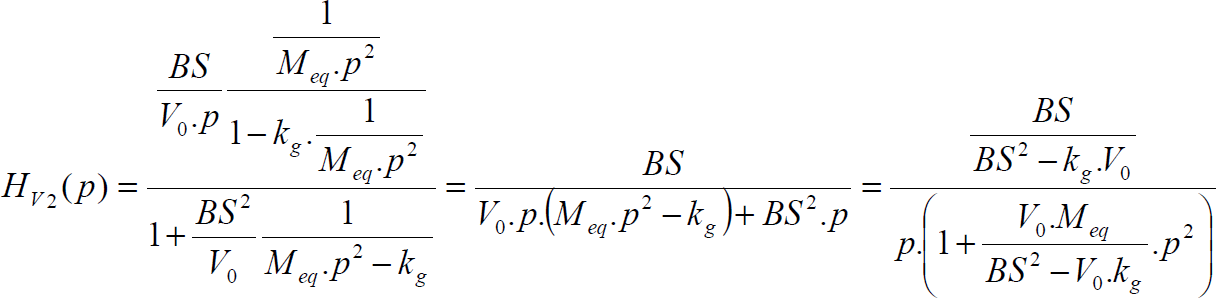
\includegraphics[width=.95\linewidth]{images/cor_05}
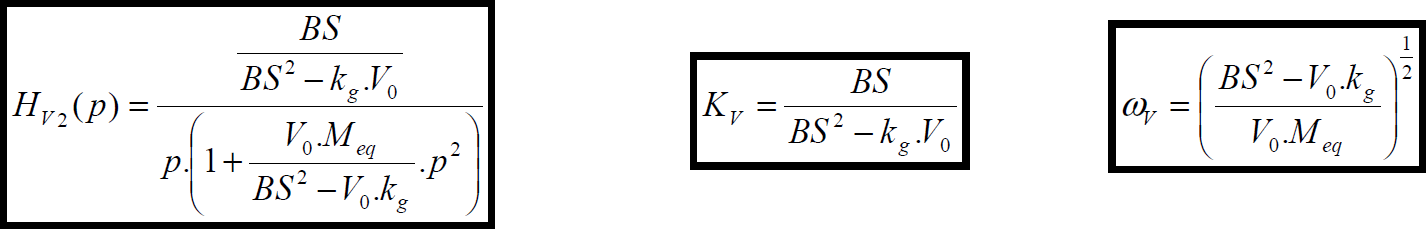
\includegraphics[width=.95\linewidth]{images/cor_06}
%\textit{}
\end{center}
\end{corrige}
\else
\fi

\textbf{$k_g$ peut maintenant être négligé.}

\subsection*{Modélisation du comportement dynamique avec prise en compte d'un débit de fuite}
Pour pallier le problème de stabilité du modèle précédemment établi, une solution possible consiste à introduire un débit de fuite au niveau du vérin. Celui-ci a pour effet de réduire artificiellement le débit réel entrant dans le vérin en fonction de la pression utile. L'expression du débit est alors : 
$q(t)=S\dot{\lambda}(t)+\dfrac{V_0}{B} \dot{p}_r(t)-\delta p_r(t)$ où $\delta$ représente le coefficient de débit de fuite.


\subparagraph{}\textit{Proposer une modification du schéma-bloc donné afin de prendre en compte le débit de fuite.}
\ifprof
\begin{corrige}
\begin{center}
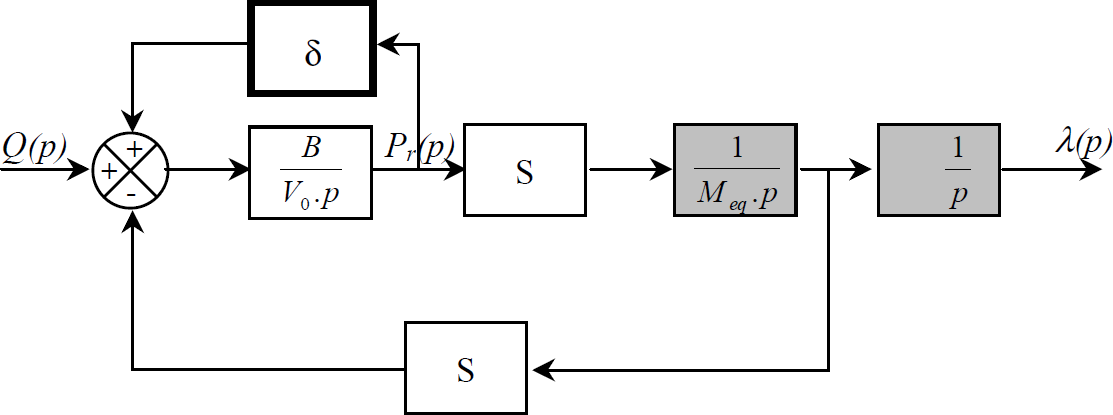
\includegraphics[width=.95\linewidth]{images/cor_07}
%\textit{}
\end{center}
\end{corrige}
\else
\fi
%\begin{center}
%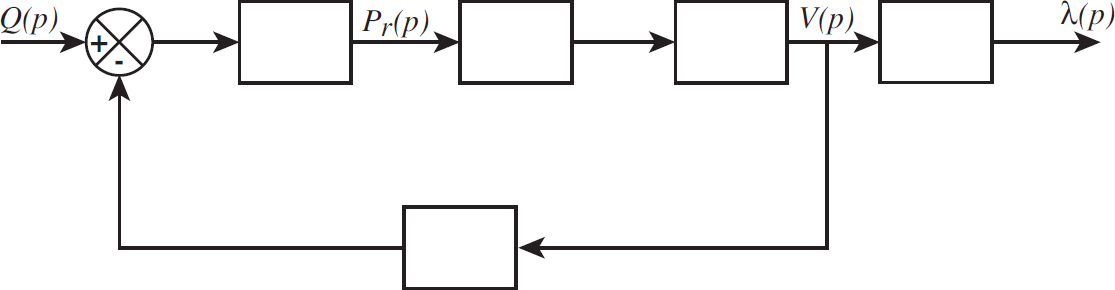
\includegraphics[width=\linewidth]{images/fig_08}
%%\textit{}
%\end{center}


\subparagraph{}\textit{Déterminer l'expression de la fonction de transfert $H_{V3}$ (telle que $\lambda(p) =  H_{V3} Q(p)$) associée au comportement dynamique du vérin ainsi modélisé. On donnera le résultat sous la forme suivante : 
$H_{V3}(p)=\dfrac{K_V}{p\left(1+a_1 p + \dfrac{p^2}{\omega_V^2} \right)}$.  
Donner l'expression de $a_1$ en fonction de $M_{eq}$, $\delta$ et $S$ et déterminer l'expression du coefficient d'amortissement $\xi_V$ du second ordre en fonction de $M_{\text{eq}}$, $\delta$, $S$, $B$ et $V_0$.}
\ifprof
\begin{corrige}
\begin{center}
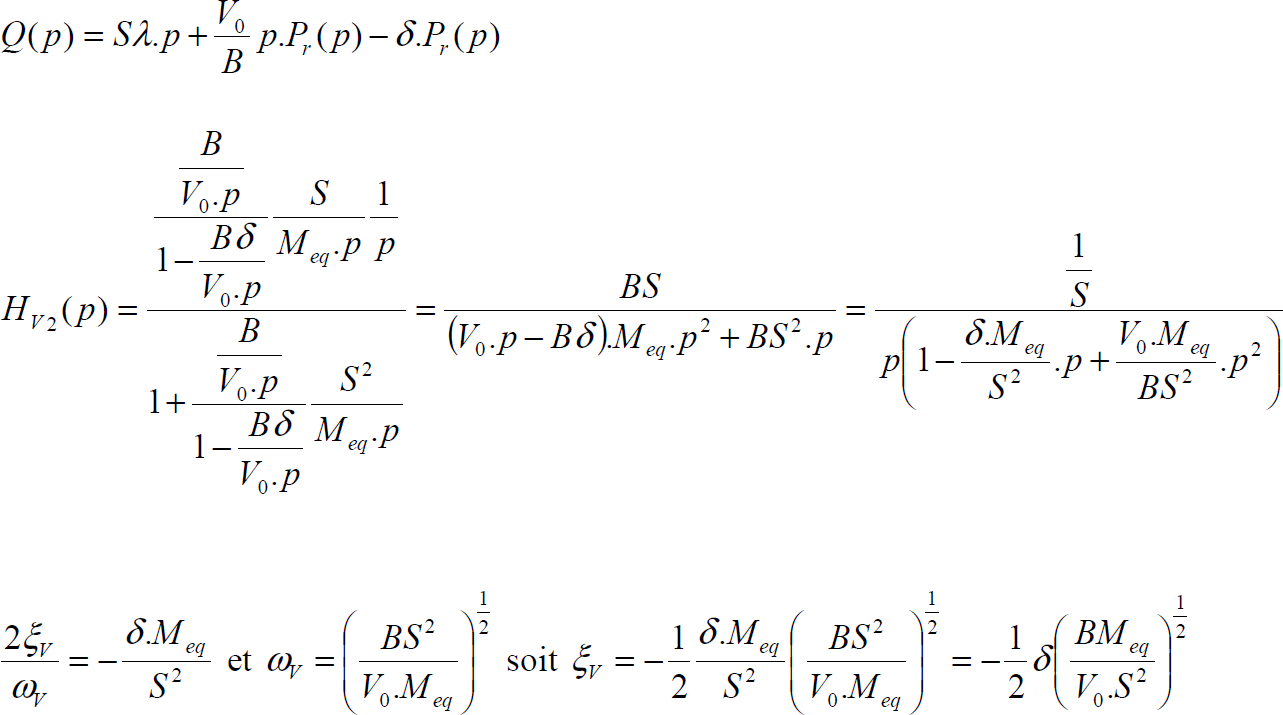
\includegraphics[width=.95\linewidth]{images/cor_08}
%\textit{}
\end{center}
\end{corrige}
\else
\fi


\subsection*{Analyse du comportement global et détermination de la valeur limite du coefficient de débit de fuite}


L'objectif de cette partie est d'analyser le comportement dynamique prévu par le modèle développé précédemment. Pour cela, on considère le système modélisé par le schéma bloc de la Figure \ref{figii.3}.


\subparagraph{}\textit{Déterminer la valeur numérique de $\omega_V$.}
\ifprof
\begin{corrige}
\end{corrige}
\else
\fi


Quels que soient les résultats obtenus précédemment, on prendra les valeurs numériques suivantes :
$C = \SI{1}{V/rad}$, $K_S = \SI{65e-4}{m^3.s^{-1}.V^{-1}}$, $K_V = \SI{1,25e3}{m^{-2}.s}$, $R = \SI{7,5}{rad/m}$.

\subparagraph{}\textit{Tracer le diagramme asymptotique de Bode de la fonction de transfert en boucle ouverte $\text{FTBO}_1$ du système asservi, avec : $M(p)=\text{FTBO}_1(p).\varepsilon(p)$}
\ifprof
\begin{corrige}
\end{corrige}
\else
\fi

\subparagraph{}\textit{Déterminer la valeur limite de $\xi_V$ assurant la stabilité du modèle. À partir de l'expression de $\xi_V$ déterminer la valeur numérique limite du coefficient de débit de fuite $\delta$.}
\ifprof
\begin{corrige}
\end{corrige}
\else
\fi

%\subsection**{Retour sur le cahier des charges}
%Le régulateur étant a priori optimisé, on réalise un essai de validation du comportement temporel de l'inclinaison de l'habitacle, le véhicule étant à l'arrêt. Le calculateur envoie un signal de consigne représentant l'évolution de la position angulaire souhaitée (de 0 à 45\degres en \SI{0,75}{s}). 
%
%\begin{center}
%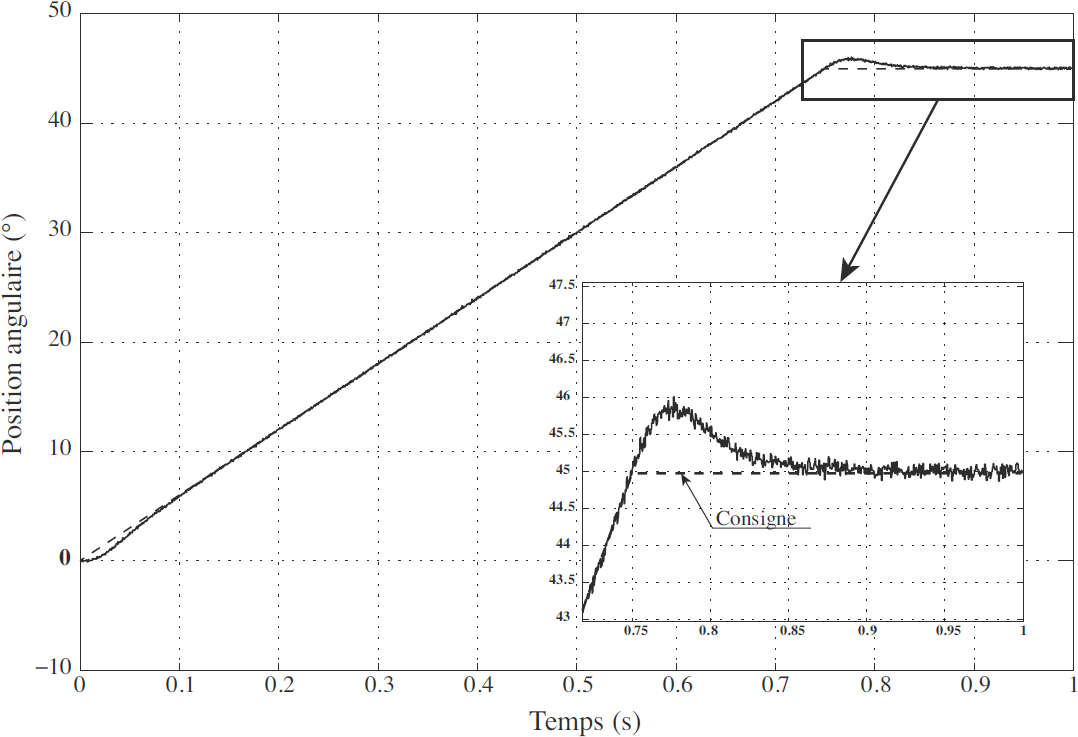
\includegraphics[width=\linewidth]{images/fig_09}
%%\textit{}
%\end{center}


\subsection*{Validation des critères principaux de la fonction technique « Contrôler le mouvement de l'habitacle~»}



\begin{obj}
L'objectif de cette partie est de définir le correcteur et de déterminer les valeurs numériques de ses paramètres caractéristiques, afin d'obtenir un asservissement en poursuite du mouvement de l'habitacle validant les critères de la fonction technique FT13 « Contrôler le mouvement de l'habitacle » qui a été proposée pour assurer la fonction technique FT1 «Modifier l'inclinaison de l'habitacle ».
\end{obj}



%III.1 —   Synthèse des résultats obtenus précédemment

On considère le schéma-blocs de la Figure \ref{fig31} avec :
 	 		 		 
 

\begin{center}
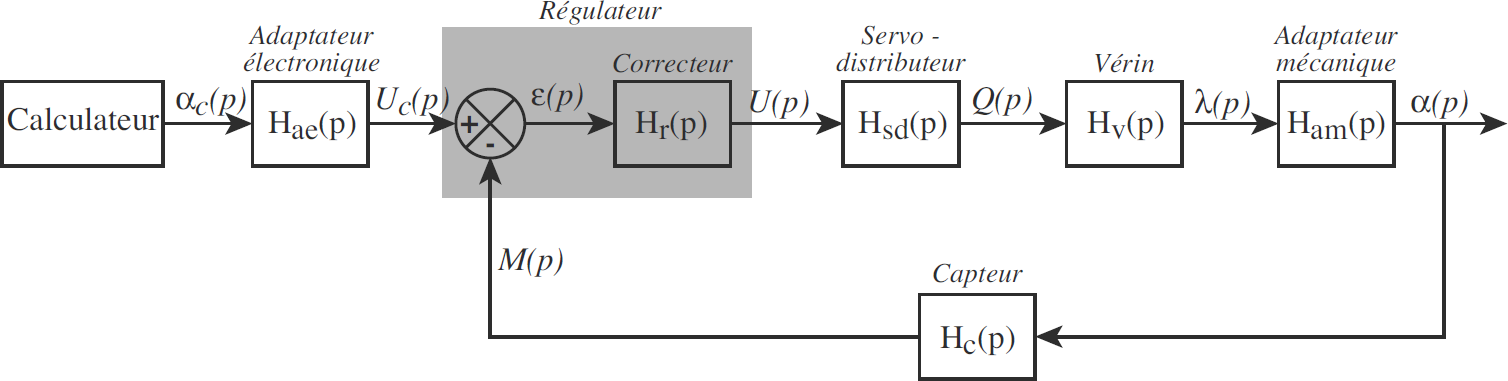
\includegraphics[width=\linewidth]{images/pt_31}
\captionof{figure}{Architecture générale du contrôle de l'orientation de l'habitacle \label{fig31}}
\end{center}



On prendra les valeurs numériques suivantes :
$C = \SI{1}{V/rad}$,
$K_S = \SI{3e-3}{m^3.s^{-1}.V^{-1}}$, 
$K_V = \SI{1,25e-3}{m^{-2}.s}$, 
$\omega_V = \SI{50}{rad.s^{-1}}$, 
$\xi_V = 0,5$, $R = \SI{7,5}{rad/m}$.


Le tableau suivant rappelle les critères et niveaux associés à la fonction technique FT13.
\begin{center}
\begin{tabular}{|p{2cm}|p{3cm}|p{2cm}|}
\hline
Fonction technique & Critères d'appréciation & Niveau \\ \hline
FT13 & Écart de traînage (entrée en rampe unitaire) & 0\degres \\ 
Contrôler le mouvement &  Écart dynamique & $<1\degres$ \\
 de l'habitacle & Temps de réponse à 5\% & $\leq \SI{0,1}{s}$  \\
 & Marge de phase & comprise entre $45\degres$  et $50\degres$  \\
 & Bande passante à \SI{-3}{dB} &  comprise entre 50 et \SI{70}{rad/s} \\
 \hline
\end{tabular}
\end{center}


 
Le temps de réponse de l'adaptateur électronique est suffisamment faible comparativement aux temps caractéristiques des autres systèmes pour que l'on puisse modéliser son comportement temporel par un gain pur $K_{ae}$.
\subparagraph{}
\textit{Donner l'expression de $K_{ae}$ pour que l'écart $\varepsilon(t)$ ait un sens.}
\ifprof
\begin{corrige}
\end{corrige}
\else
\fi



\subsubsection*{Première correction}

Afin de répondre au critère du cahier des charges concernant la précision statique du système, on choisit de placer un intégrateur comme premier correcteur :  $H_r(p)=\dfrac{K_i}{p}$.



\subparagraph{}
\textit{On donne le diagramme de Bode de la fonction de transfert en boucle ouverte $\text{FTBO}_2$ du système asservi pour $K_i = 1$ et telle que $M(p) = \text{FTBO}_2(p) \varepsilon(p)$. Déterminer, en expliquant clairement la méthode employée, la valeur de $K_i$ qui permet d'obtenir la dynamique souhaitée.}
\ifprof
\begin{corrige}
\end{corrige}
\else
\fi

\begin{center}
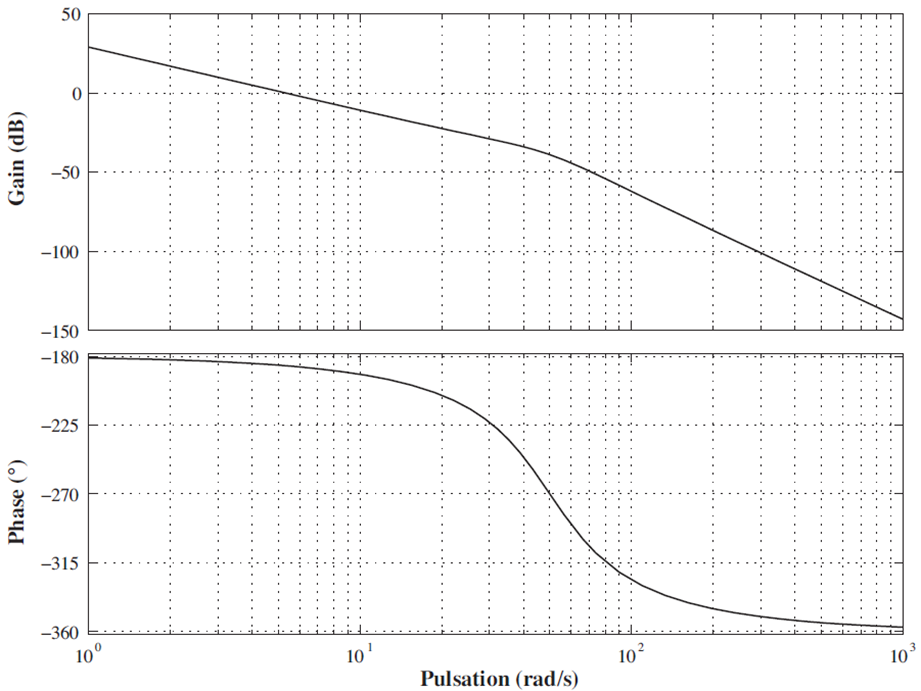
\includegraphics[width=\linewidth]{images/pt_37}
\end{center}

\subparagraph{}
\textit{Combien de correcteurs à avance de phase réglés pour apporter chacun 50\degres au maximum faudrait-il incorporer dans le régulateur pour satisfaire le critère de marge de phase du cahier des charges ?
}
\ifprof
\begin{corrige}
\end{corrige}
\else
\fi


On souhaite réaliser une simulation du comportement temporel du système ainsi corrigé pour un passage de 0 à 45\degres de l'habitacle en \SI{0,75}{s}. Le signal de consigne est donné sur la Figure \ref{fig32}. Le logiciel de simulation ne possède pas de bloc de signal d'entrée correspondant à ce type de fonction, mais il est possible d'utiliser des blocs de type « rampe » possédant les critères :
\begin{itemize}
\item pente de la rampe ;
\item instant de départ de la rampe.
\end{itemize}
 

\begin{center}
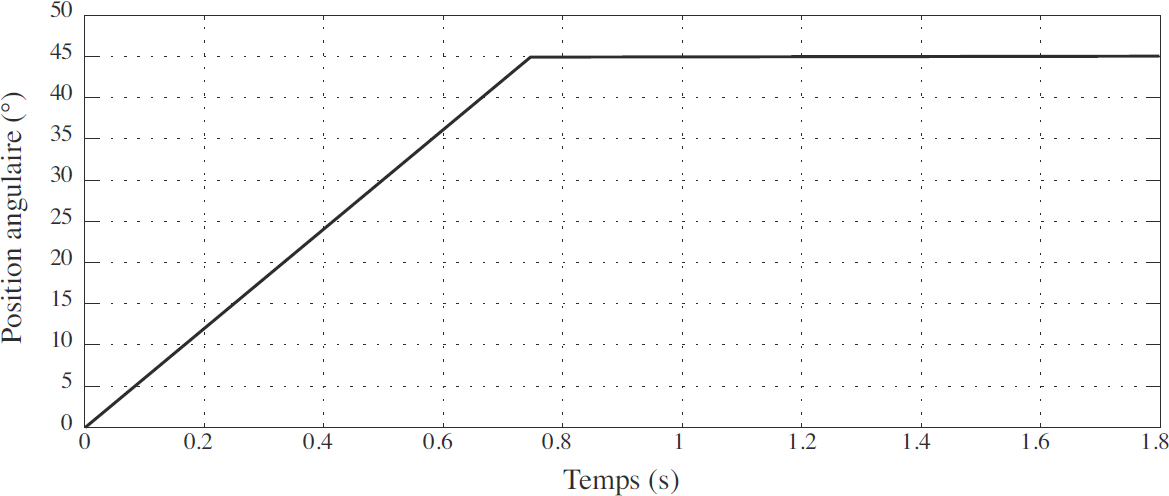
\includegraphics[width=\linewidth]{images/pt_32}
\captionof{figure}{Signal de consigne pour une simulation d'une rotation de 0 à 45\degres en \SI{0,75}{s} \label{fig32}}
\end{center}





\subparagraph{}
\textit{Donner les paramètres à entrer dans les 2 blocs de type « rampes » et préciser l'opération mathématique à effectuer entre les deux blocs afin d'obtenir le signal présenté sur la Figure \ref{fig32}}
\ifprof
\begin{corrige}
\end{corrige}
\else
\fi



La réponse obtenue par la simulation est présentée sur la Figure \ref{fig33}.

\begin{center}
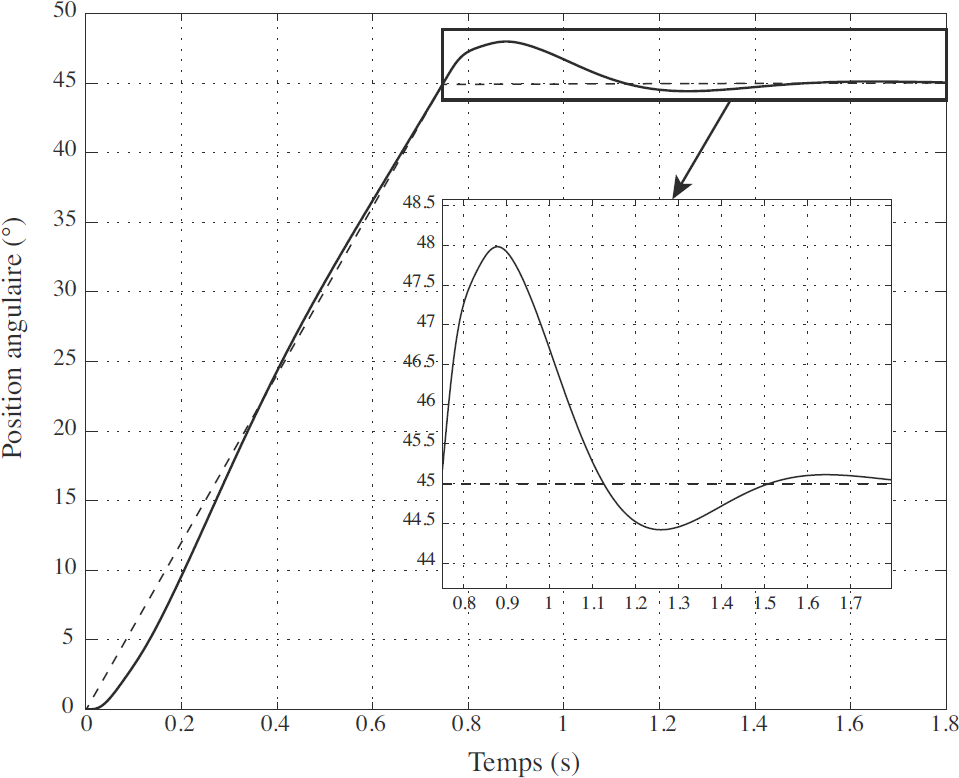
\includegraphics[width=\linewidth]{images/pt_33}
\captionof{figure}{Résultat de la simulation du passage de 0 à 45\degres en \SI{0,75}{s} \label{fig33}}
\end{center}


\subparagraph{}
\textit{Quels sont les critères non satisfaits ?}
\ifprof
\begin{corrige}
\end{corrige}
\else
\fi


\subsubsection*{Deuxième correction}

Plusieurs réglages du correcteur précédent ont été réalisés mais aucun n'a pu apporter satisfaction quant aux différents critères du cahier des charges. Le problème de fond ici est lié au fait que la pulsation de coupure $\omega_v$ du mode de second ordre de la fonction de transfert du vérin est inférieure à la pulsation à \SI{0}{dB} souhaitée pour garantir une dynamique suffisante du système bouclé. On souhaite donc augmenter la valeur de la pulsation de coupure $\omega_v$ afin de garantir au moins deux décades d'écart avec la pulsation à \SI{0}{dB} de la fonction de transfert en boucle ouverte du système.

\subparagraph{}
\textit{Quelle valeur de diamètre du vérin permet de vérifier la condition précédente. Cette valeur est-elle réaliste ?}
\ifprof
\begin{corrige}
\end{corrige}
\else
\fi



On décide alors de remédier à ce problème par un filtre électronique du second ordre de type Notch de fonction de transfert : $H_N(p)=\dfrac{1+\dfrac{2\xi_np}{\omega_n}+\dfrac{p^2}{\omega_n^2}}{1+\dfrac{2\xi_dp}{\omega_d}+\dfrac{p^2}{\omega_d^2}}$.
 
Le réglage optimum du correcteur doit compenser parfaitement le mode de second ordre de la fonction de transfert du vérin. Pour cela, on effectue un essai afin d'identifier les caractéristiques de ce mode. Aucun réglage spécifique du débit de fuite n'a été réalisé, la compensation du mode rendant inutile cette étape.

Une tension de consigne $u_e(t) = 0,02 u(t)$ (avec $u(t)$ l'échelon unitaire) est envoyée en entrée du servo-distributeur. Une génératrice tachymétrique, dont le comportement est modélisé par un gain pur $K_{gt} = \SI{2}{V.rad^{-1}.s}$, mesure la vitesse de rotation de l'habitacle. Cette tension est notée $m_{\omega}(t)$. Le résultat de cet essai est donné sur la Figure de la question 34 du Cahier Réponses.

\subparagraph{}
\textit{Compléter sur le Cahier Réponses le schéma-blocs représentant cet essai et déterminer la fonction de transfert $H_{\text{essai}}$ telle que : $M_{\Omega}(p) = H_{\text{essai}}(p).U_e(p)$.}
\ifprof
\begin{corrige}
\end{corrige}
\else
\fi


\subparagraph{}
\textit{En vous aidant du graphe de la Figure \ref{fig34}, déterminer les valeurs numériques expérimentales de $\omega_v$ et $\xi_v$ à partir de la courbe obtenue expérimentalement tracée sur le Cahier Réponses.}
\ifprof
\begin{corrige}
\end{corrige}
\else
\fi

\subparagraph{}
\textit{Quels inconvénients sur le comportement réel du système peuvent découler de cette méthode consistant à vouloir compenser le mode de second ordre de la fonction de transfert du vérin par ce type de filtre électronique ?}
\ifprof
\begin{corrige}
\end{corrige}
\else
\fi


\begin{center}
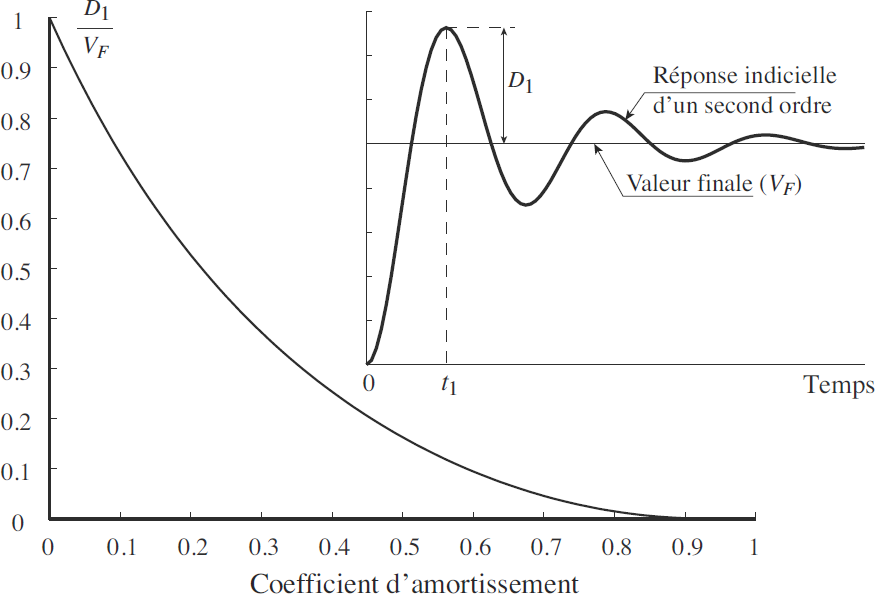
\includegraphics[width=.6\linewidth]{images/pt_34}
\captionof{figure}{Évolution du premier dépassement relatif à la valeur finale en fonction du coefficient d'amortissement (pour une fonction de transfert du second ordre) \label{fig34}}
\end{center}
 

On suppose par la suite que le numérateur du filtre Notch compense parfaitement le mode de second ordre de la fonction de transfert du vérin. On adopte les caractéristiques suivantes pour le dénominateur :
\begin{itemize}
\item $\omega_d = \SI{1000}{rad.s^{-1}}$ ;
\item $\xi_d = 1$.
\end{itemize}

Afin de satisfaire le critère de précision statique du cahier des charges on place un premier correcteur de type intégrateur non unitaire de fonction de transfert : $H_{\text{cor2}}(p)=\dfrac{K_{\Omega}}{p}$.

La valeur de $K_{\Omega}$ est déterminée afin d'obtenir une pulsation à \SI{0}{dB} de la fonction de transfert en boucle ouverte de $\SI{65}{rad.s^{-1}}$. Le diagramme de Bode de cette fonction de transfert est donné sur la Figure \ref{fig35}.

\begin{center}
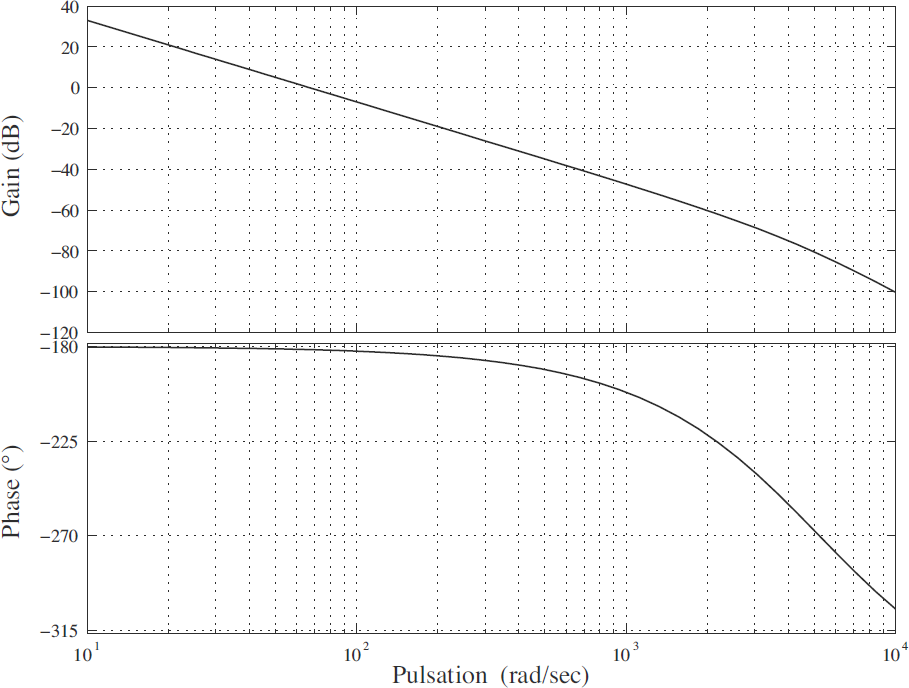
\includegraphics[width=\linewidth]{images/pt_35}
\captionof{figure}{Diagramme de Bode de la Fonction de Transfert en Boucle Ouverte après correction Intégrale \label{fig35}}
\end{center}

On complète le régulateur par un correcteur à avance de phase de fonction de transfert : $H_{\text{av}}(p)=K_{\text{av}}\dfrac{1+a_{\text{av}}\tau_{\text{av}}p}{1+\tau_{\text{av}}p}$ avec $a_{\text{av}}>1$.

\subparagraph{}
\textit{Déterminer les valeurs approximatives des paramètres $a_{av}$, $\tau_{\text{av}}$ et $K_{\text{av}}$ qui permettent de satisfaire le critère de marge de phase du cahier des charges tout en conservant une pulsation à \SI{0}{dB} de \SI{65}{rad.s^{-1}}.}
\ifprof
\begin{corrige}
\end{corrige}
\else
\fi


Le régulateur étant a priori optimisé, on réalise un essai de validation du comportement temporel de l'inclinaison de l'habitacle, le véhicule étant à l'arrêt. Le calculateur envoie un signal de consigne représentant l'évolution de la position angulaire souhaitée (de 0 à 45\degres en \SI{0,75}{s}). La tension délivrée par le capteur angulaire est récupérée par un convertisseur analogique-numérique afin de tracer sur un ordinateur l'évolution temporelle de l'inclinaison de l'habitacle mesurée en degrés. Les deux courbes sont données sur la Figure \ref{fig36}.

\subparagraph{}
\textit{Quels sont les critères du cahier des charges validés ?}
\ifprof
\begin{corrige}
\end{corrige}
\else
\fi


\begin{center}
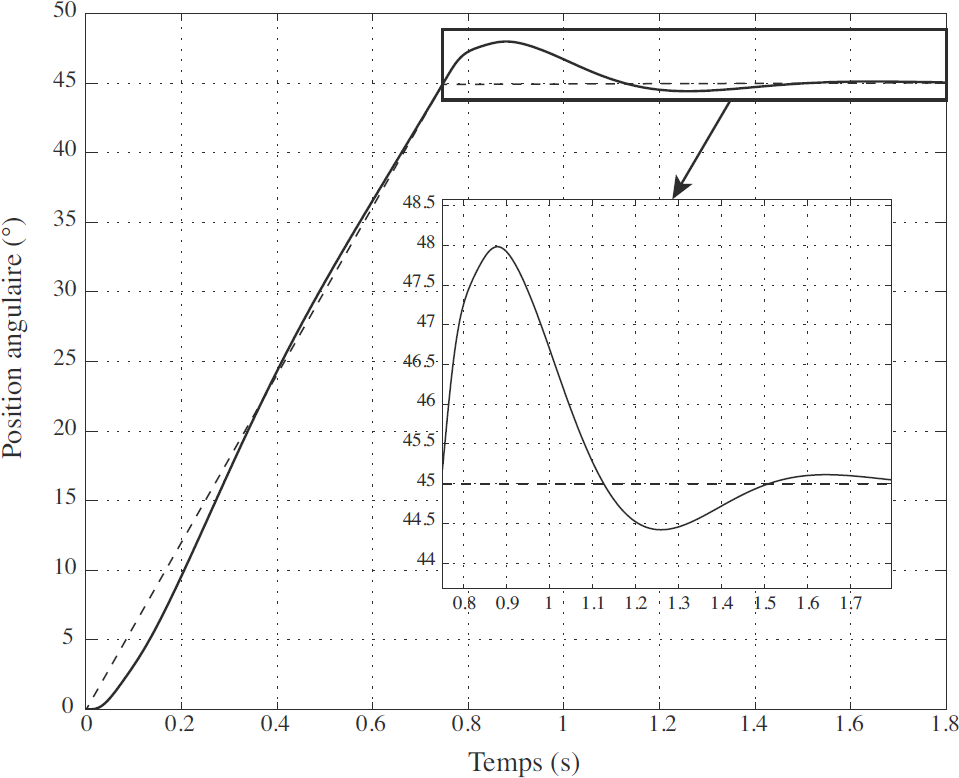
\includegraphics[width=.6\linewidth]{images/pt_33}
\captionof{figure}{Essai de validation : passage de 0 à 45\degres en \SI{0,75}{s} \label{fig36}}
\end{center}

\begin{center}
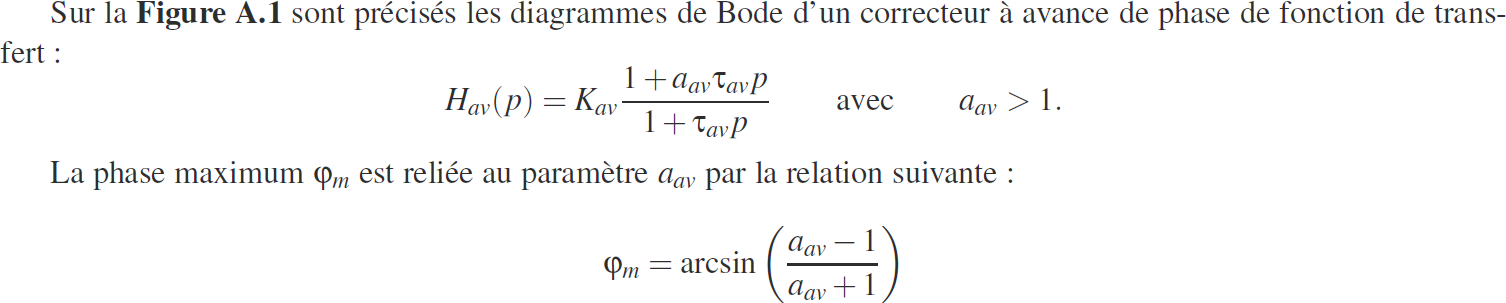
\includegraphics[width=\linewidth]{images/pt_ann_01}

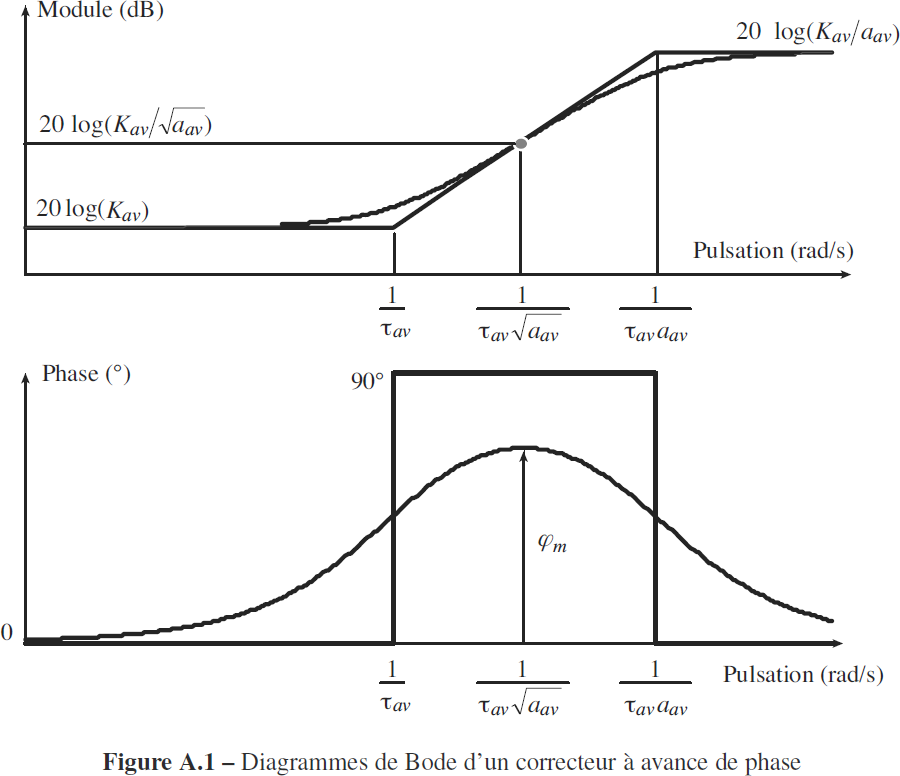
\includegraphics[width=.9\linewidth]{images/pt_ann_02}
\end{center}

%%%%%%%%%%%%%%%%%%%%%%%%%%%%%%%%%%%%%%%%%%%%%%%%%%%

\ifprof
\end{multicols}
\else
\end{multicols}
\fi


\ifprof
\else


\begin{center}
%\includegraphics[width=\linewidth]{ecart}
%\textit{}
\end{center}

\begin{center}
%\includegraphics[width=.9\linewidth]{PositionQuille}
\end{center}


\fi
%
%\end{document}
%
%\subparagraph{}\textit{}
%\ifprof
%\begin{corrige}
%\end{corrige}
%\else
%\fi
%
%\begin{center}
%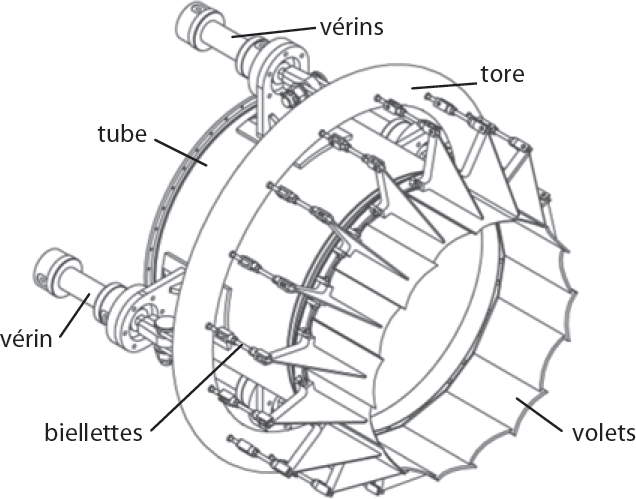
\includegraphics[width=\linewidth]{fig_04}
%%\textit{}
%\end{center}

